\documentclass[
 size=14pt,
 paper=smartboard, %a4paper, smartboard, screen
 mode=present, %present, handout, print
 display=slides, % slidesnotes, notes, slides
% nohandoutpagebreaks,
% pauseslide,
style=tuliplab,
% nopagebreaks,clock
% hlentries=true,
% hlsections = true,
pauseslide,
fleqn,leqno]{powerdot}

\hypersetup{pdfpagemode=FullScreen}
% \usepackage[toc,highlight,blackslide,slidesonly,sounds,HA]{HA-prosper}

\usepackage{graphicx}
\usepackage{subfigure}
\usepackage{amssymb}
\usepackage{amsmath} 
\usepackage{rotating}
\usepackage{boxedminipage}
\usepackage{media9}
\usepackage{rotate}
\usepackage{calc}
\usepackage[absolute]{textpos}
\usepackage{psfrag,overpic}
\usepackage{fouriernc}
\usepackage{pstricks,pst-node,pst-text,pst-3d,pst-grad}
\usepackage{moreverb,epsfig,color,subfigure}
\usepackage{color}
\usepackage{pstricks}
\usepackage{pstricks-add}
\usepackage{pst-text}
\usepackage{pst-node, pst-tree}
\usepackage{booktabs}
\usepackage{etex}
\usepackage{breqn}
\usepackage{multirow}
\usepackage{gitinfo2}


\usepackage{listings}
\lstset{frameround=fttt, 
frame=trBL, 
stringstyle=\ttfamily,
backgroundcolor=\color{yellow!20},
basicstyle=\footnotesize\ttfamily}
\lstnewenvironment{code}{
\lstset{frame=single,escapeinside=`',
backgroundcolor=\color{yellow!20},
basicstyle=\footnotesize\ttfamily}
}{}


\usepackage{fouriernc}
\usepackage{hyperref}

%%%%%%%%%%%%%%%%%%%%%%%%%%%%%%%%%%%%%%%%%%%%%%%%%%%%%%%%%%%%%%%%%%%%%%%%
% title
% TODO: Customize to your Own Title, Name, Address
%
\title{FLIP 00 mid-term Presentation}
\author{
XiaoXichang
\\
HuNan University 
% \href{mailto:gangli@acm.org}{gangli@acm.org}
% \and % more authors
}
\date{October 27, 2019}


\begin{document}

\maketitle 

\begin{slide}[toc=,bm=]{Outline}
\tableofcontents[content=sections]
\end{slide}

\section{Introduction}

\begin{slide}{Problem Description}
  \begin{itemize}
    \item  searching the relation from different varieties 
  \end{itemize}
\end{slide}


\section{Data Description}


\begin{slide}{Data Description}
\begin{itemize}
\item there are 15 attributes,including 1 class attribute and 14 feature attributes
\item the part description of the data is shown in the following figure .
\end{itemize}
\end{slide}

\begin{slide}{The part description of the data}
	\vspace*{10pt}
	\begin{figure}[htbp]
		\centering
		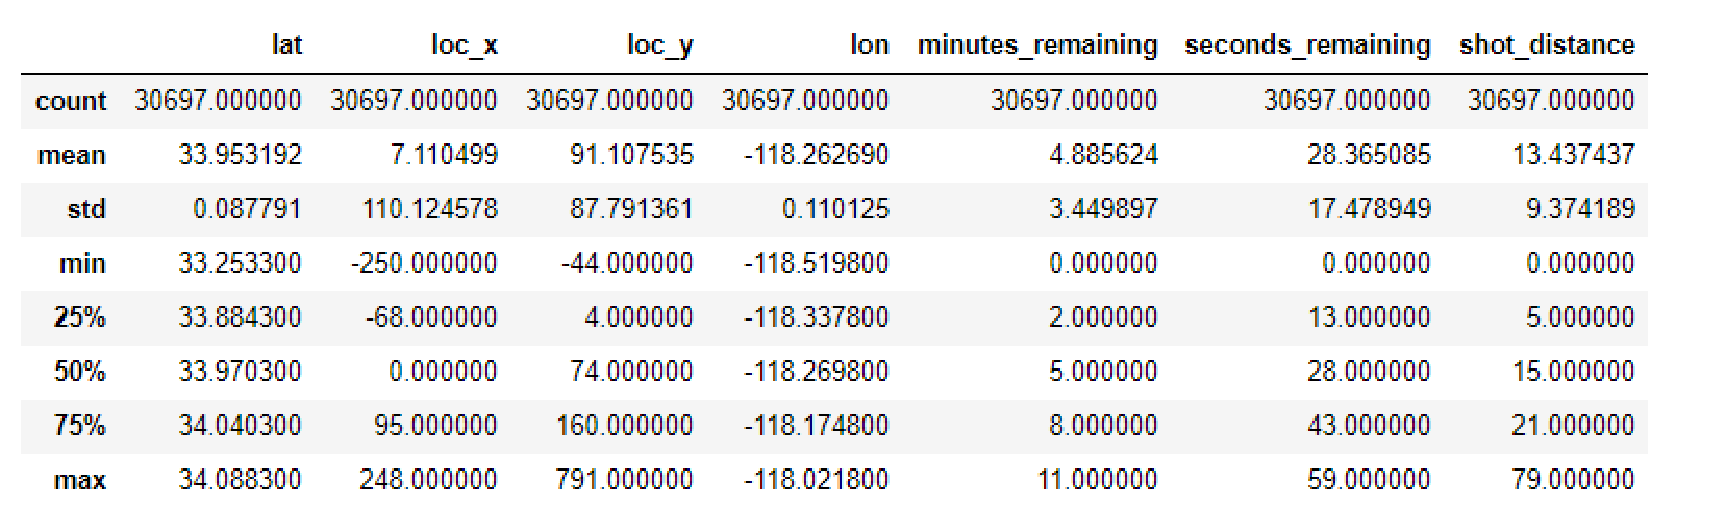
\includegraphics[scale=0.4]{1.eps}
		\caption{the part description of the data}
	\end{figure}
\end{slide}


\begin{slide}{The part description of the data}
	\vspace*{10pt}
	\begin{figure}[htbp]
		\centering
		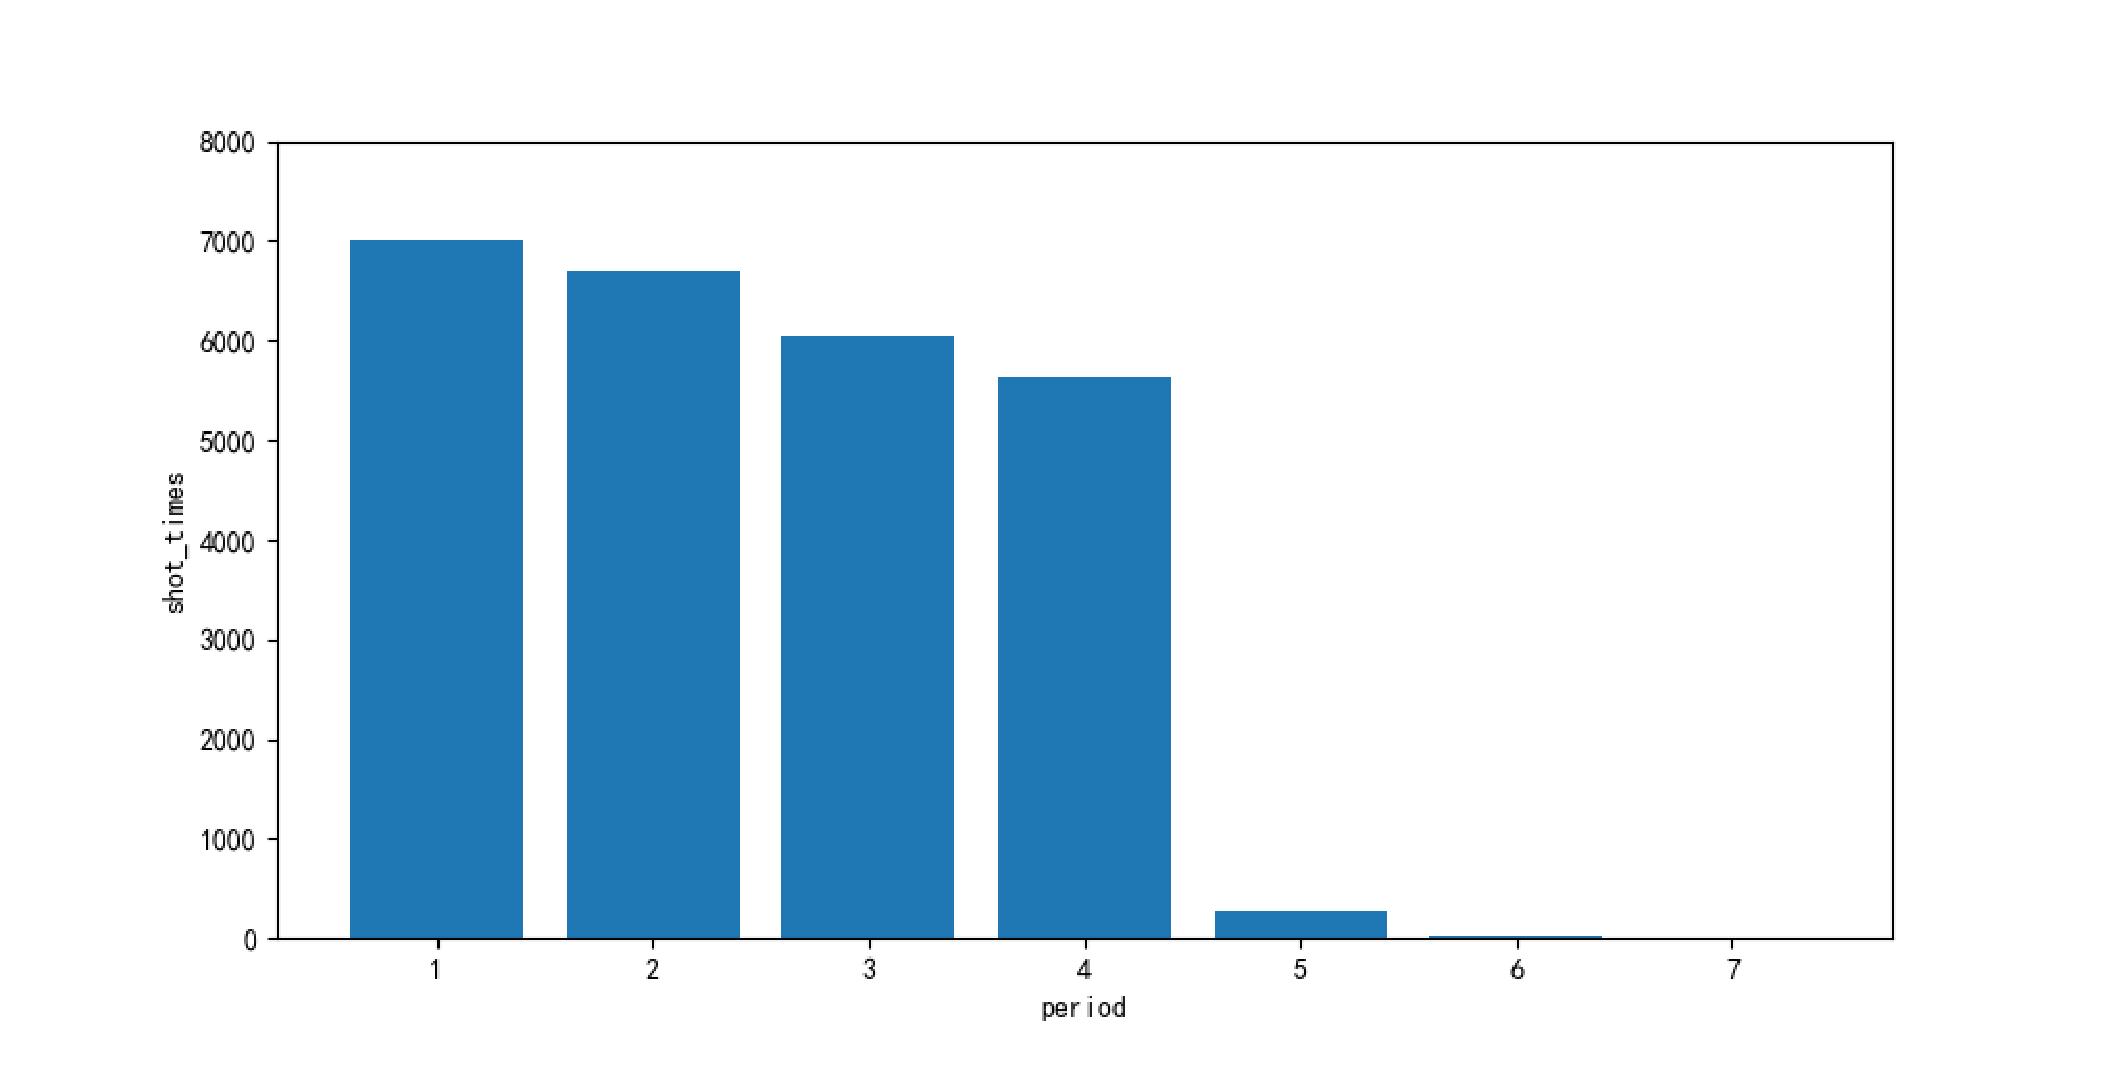
\includegraphics[scale=0.4]{o.eps}
		\caption{the part description of the data}
	\end{figure}
\end{slide}

\section{Conclusion}
	
\begin{slide}{conclusion}
	Conclusion
	
	\begin{itemize}
		\item  It is possible to bulid a classfication model to predict houses for different demands of people.
	\end{itemize}
\end{slide}
%%==========================================================================================
% TODO: Contact Page
\begin{wideslide}[toc=,bm=]{}
\vspace*{100pt}
\begin{center} 
\hspace*{100pt}	
{\Huge Thank you \& Question }
\end{center}	
\end{wideslide}



\end{document}

\endinput